
% global preamble
%Style
\documentclass[12pt]{article}
\usepackage[top=1in, bottom=1in, left=1in, right=1in]{geometry}
\parindent 22pt
\usepackage{fancyhdr}

%Packages
\usepackage{adjustbox}
\usepackage{amsmath}
\usepackage{amsfonts}
\usepackage{amssymb}
\usepackage{bm}
\usepackage[table]{xcolor}
\usepackage{tabu}
\usepackage{makecell}
\usepackage{longtable}
\usepackage{multirow}
\usepackage[normalem]{ulem}
\usepackage{etoolbox}
\usepackage{graphicx}
\usepackage{tabularx}
\usepackage{ragged2e}
\usepackage{booktabs}
\usepackage{caption}
\usepackage{fixltx2e}
\usepackage[para, flushleft]{threeparttablex}
\usepackage[capposition=top]{floatrow}
\usepackage{subcaption}
\usepackage{pdfpages}
\usepackage{pdflscape}
\usepackage{natbib}
\usepackage{bibunits}
\definecolor{maroon}{HTML}{990012}
\usepackage[colorlinks=true,linkcolor=maroon,citecolor=maroon,urlcolor=maroon,anchorcolor=maroon]{hyperref}
\usepackage{marvosym}
\usepackage{makeidx}
\usepackage{tikz}
\usetikzlibrary{shapes}
\usepackage{setspace}
\usepackage{enumerate}
\usepackage{rotating}
\usepackage{epstopdf}
\usepackage[titletoc]{appendix}
\usepackage{framed}
\usepackage{comment}
\usepackage{xr}
\usepackage{titlesec}
\usepackage{footnote}
\usepackage{longtable}
\newlength{\tablewidth}
\setlength{\tablewidth}{9.3in}
\setcounter{secnumdepth}{4}

\titleformat{\paragraph}
{\normalfont\normalsize\bfseries}{\theparagraph}{1em}{}
\titlespacing*{\paragraph}
{0pt}{3.25ex plus 1ex minus .2ex}{1.5ex plus .2ex}
\makeatletter
\pretocmd\start@align
{%
  \let\everycr\CT@everycr
  \CT@start
}{}{}
\apptocmd{\endalign}{\CT@end}{}{}
\makeatother
%Watermark
\usepackage[printwatermark]{xwatermark}
\usepackage{lipsum}
\definecolor{lightgray}{RGB}{220,220,220}
%\newwatermark[allpages,color=lightgray,angle=45,scale=3,xpos=0,ypos=0]{Preliminary Draft}

%Further subsection level
\usepackage{titlesec}
\setcounter{secnumdepth}{4}
\titleformat{\paragraph}
{\normalfont\normalsize\bfseries}{\theparagraph}{1em}{}
\titlespacing*{\paragraph}
{0pt}{3.25ex plus 1ex minus .2ex}{1.5ex plus .2ex}

\setcounter{secnumdepth}{5}
\titleformat{\subparagraph}
{\normalfont\normalsize\bfseries}{\thesubparagraph}{1em}{}
\titlespacing*{\subparagraph}
{0pt}{3.25ex plus 1ex minus .2ex}{1.5ex plus .2ex}

%Functions
\DeclareMathOperator{\cov}{Cov}
\DeclareMathOperator{\var}{Var}
\DeclareMathOperator{\plim}{plim}
\DeclareMathOperator*{\argmin}{arg\,min}
\DeclareMathOperator*{\argmax}{arg\,max}

%Math Environments
\newtheorem{theorem}{Theorem}[section]
\newtheorem{claim}[theorem]{Claim}
\newtheorem{assumption}[theorem]{Assumption}
\newtheorem{definition}[theorem]{Definition}
\newtheorem{hypothesis}[theorem]{Hypothesis}
\newtheorem{property}[theorem]{Property}
\newtheorem{example}[theorem]{Example}
\newtheorem{condition}[theorem]{Condition}
\newtheorem{result}[theorem]{Result}
\newenvironment{proof}{\paragraph{Proof:}}{\hfill$\square$}

%Commands
\newcommand\independent{\protect\mathpalette{\protect\independenT}{\perp}}
\def\independenT#1#2{\mathrel{\rlap{$#1#2$}\mkern2mu{#1#2}}}
\newcommand{\overbar}[1]{\mkern 1.5mu\overline{\mkern-1.5mu#1\mkern-1.5mu}\mkern 1.5mu}
\newcommand{\equald}{\ensuremath{\overset{d}{=}}}
\captionsetup[table]{skip=10pt}
%\makeindex


\newcolumntype{L}[1]{>{\raggedright\let\newline\\\arraybackslash\hspace{0pt}}m{#1}}
\newcolumntype{C}[1]{>{\centering\let\newline\\\arraybackslash\hspace{0pt}}m{#1}}
\newcolumntype{R}[1]{>{\raggedleft\let\newline\\\arraybackslash\hspace{0pt}}m{#1}}



%Logo
%\AddToShipoutPictureBG{%
%  \AtPageUpperLeft{\raisebox{-\height}{\includegraphics[width=1.5cm]{uchicago.png}}}
%}

\newcolumntype{L}[1]{>{\raggedright\let\newline\\\arraybackslash\hspace{0pt}}m{#1}}
\newcolumntype{C}[1]{>{\centering\let\newline\\\arraybackslash\hspace{0pt}}m{#1}}
\newcolumntype{R}[1]{>{\raggedleft\let\newline\\\arraybackslash\hspace{0pt}}m{#1}} 

\newcommand{\mr}{\multirow}
\newcommand{\mc}{\multicolumn}

%\newcommand{\comment}[1]{}


\begin{document}

\title{Description of Reggio Variables}
\author{Reggio Team}
\date{Original version: Monday 18$^{\text{th}}$ July, 2016 \\ Current version: \today \\ \vspace{1em} Time: \currenttime}
\maketitle

\tableofcontents

\doublespace

\section{Overview}
\label{sec:overview}
This document compiles information on the variables in the Reggio dataset. The information presented includes (1) an explanation of relevant variables by broad category (e.g. health outcomes), (2) descriptive statistics, (3) a tabulation of missing observations, and (4) a discussion of any issues with the variables. 


\section{Non-cognitive Variables}
\label{sec:non-cognitive}
\setlength{\tabcolsep}{20pt}

\begin{table}[H]
\rowcolors{3}{gray!7}{white}
	\begin{center}

	\scalebox{0.9}{
	\begin{threeparttable}
	\caption{Availability of variables by cohort}
		\begin{tabular}{L{5.5cm}C{2cm} C{2cm} C{2cm}} \hline
															& \textbf{Children Cohort} 			& \textbf{Adol Cohort} 		& \textbf{Adult Cohort} 		\\ 
		\hline	
		\textbf{Depression Score}							&									& \checkmark				& \checkmark					\\
		\textbf{Locus of Control}								&									& \checkmark				& \checkmark					\\
		%Caregiver Locus of Control							& \checkmark						&\checkmark															\\
		\textbf{Optimistic outlook on life}						&									& \checkmark				& \checkmark					 \\

		\textbf{SDQ Scores} \footnotemark \footnotemark		&									&							&								\\
		\quad \quad SDQ Composite score						& \checkmark						& \checkmark				&								\\
		\quad \quad SDQ Emotional score						& \checkmark						& \checkmark				&								\\
		\quad \quad SDQ Conduct score							& \checkmark					& \checkmark				&								\\
		\quad \quad SDQ Hyper score							& \checkmark						& \checkmark				&								\\
		\quad \quad SDQ Peer problems score					& \checkmark						& \checkmark				&								\\
		\quad \quad SDQ Pro-social score						&\checkmark							& \checkmark				&								\\

		\textbf{Satisfaction variables}							&									&							&								 \\
		\quad \quad Satisfied with income						& 									&							& \checkmark					\\
		\quad \quad Satisfied with work						& 									&							& \checkmark					\\	
		\quad \quad Satisfied with health						&									& \checkmark				& \checkmark					\\
		\quad \quad Satisfied with family						&									& \checkmark				& \checkmark					\\
		\quad \quad Satisfied with school						&									& \checkmark 				&								\\
		%\quad \quad Satisfied with education					&									& \checkmark 				&								\\
		
		\textbf{Reciprocity variables}							&									&							&								\\
		\quad \quad Return favor								&									& \checkmark				& \checkmark					 \\
		\quad \quad Put someone in difficulty					&									& \checkmark				& \checkmark					 \\	
		\quad \quad Help someone kind to me					&									& \checkmark				& \checkmark					 \\
		\quad \quad Insult back								&									& \checkmark				& \checkmark					 \\

		
		\hline
		\end{tabular}

		\begin{tablenotes}
		\singlespace
		\footnotesize{
			\item [1] The dataset includes the childSDQ score for children. This score is reported by mothers. \\
			\item [2] The dataset includes data on both childSDQ and SDQ scores for Adolescents. The childSDQ is reported by the mother, and the SDQ is reported by adolescent.	
		}
		\end{tablenotes}
	\end{threeparttable}
	}
	\end{center}
\end{table}
\setcounter{footnote}{0}

 \clearpage

\begin{landscape}
\singlespace
\setlength{\tabcolsep}{2pt}
\begin{center}
\scriptsize{
\begin{longtable}{L{5cm} c c c p{.5cm} c c c p{.5cm} c c c p{.5cm} c c c p{.5cm} c c c}
\hline
\multicolumn{20}{L{20cm}}{\textbf{Note:} Unconditional means are reported for each variable by cohort and city. Standard Deviations are reported in italics below each mean estimates.}
\endfoot
\caption{Mean and Standard Deviation for Non-cognitive variables by city and cohort} \label{table:Desc_N} \\
& \multicolumn{3}{c}{\textbf{Children}} & & \multicolumn{3}{c}{\textbf{Adolescents}} & & \multicolumn{3}{c}{\textbf{Adults 30}} & & \multicolumn{3}{c}{\textbf{Adults 40}} & & \multicolumn{3}{c}{\textbf{Adults 50}}\\
& \scriptsize{Reggio} & \scriptsize{Parma}& \scriptsize{Padova} & & \scriptsize{Reggio} & \scriptsize{Parma}& \scriptsize{Padova} & & \scriptsize{Reggio} & \scriptsize{Parma}& \scriptsize{Padova} & & \scriptsize{Reggio} & \scriptsize{Parma}& \scriptsize{Padova} & & \scriptsize{Reggio} & \scriptsize{Parma}& \scriptsize{Padova}\\
\hline \endhead
Depression Score - positive & . &         . &         . & &     37.14 &     37.89 &     38.61 & &     37.80 &     39.21 &     38.94 & &     38.83 &     39.51 &     39.10 & &     37.62 &     38.04 &     35.79 \\*
& $\mathit{        .}$ & $\mathit{        .}$ & $\mathit{        .}$ & & $\mathit{     6.51}$ & $\mathit{     5.03}$ & $\mathit{     5.95}$ & & $\mathit{     5.83}$ & $\mathit{     5.92}$ & $\mathit{     5.55}$ & & $\mathit{     5.87}$ & $\mathit{     5.30}$ & $\mathit{     5.61}$ & & $\mathit{     5.16}$ & $\mathit{     4.69}$ & $\mathit{     6.06}$ \\[1.6em]
Locus of Control - positive & . &         . &         . & &      0.06 &     -0.15 &      0.07 & &      0.09 &     -0.23 &      0.26 & &      0.15 &     -0.11 &      0.15 & &      0.12 &     -0.40 &     -0.06 \\*
& $\mathit{        .}$ & $\mathit{        .}$ & $\mathit{        .}$ & & $\mathit{     0.71}$ & $\mathit{     0.82}$ & $\mathit{     0.73}$ & & $\mathit{     0.74}$ & $\mathit{     0.97}$ & $\mathit{     0.79}$ & & $\mathit{     0.82}$ & $\mathit{     0.87}$ & $\mathit{     0.82}$ & & $\mathit{     0.83}$ & $\mathit{     0.91}$ & $\mathit{     0.91}$ \\[1.6em]
Optimistic Look on Life & . &         . &         . & &      0.67 &      0.69 &      0.56 & &      0.55 &      0.55 &      0.61 & &      0.59 &      0.30 &      0.46 & &      0.20 &      0.19 &      0.23 \\*
& $\mathit{        .}$ & $\mathit{        .}$ & $\mathit{        .}$ & & $\mathit{     0.47}$ & $\mathit{     0.46}$ & $\mathit{     0.50}$ & & $\mathit{     0.50}$ & $\mathit{     0.50}$ & $\mathit{     0.49}$ & & $\mathit{     0.49}$ & $\mathit{     0.46}$ & $\mathit{     0.50}$ & & $\mathit{     0.40}$ & $\mathit{     0.39}$ & $\mathit{     0.42}$ \\[1.6em]
SDQ Composite & . &         . &         . & &      9.22 &      8.21 &      8.89 & &         . &         . &         . & &         . &         . &         . & &         . &         . &         . \\*
& $\mathit{        .}$ & $\mathit{        .}$ & $\mathit{        .}$ & & $\mathit{     5.33}$ & $\mathit{     4.89}$ & $\mathit{     5.15}$ & & $\mathit{        .}$ & $\mathit{        .}$ & $\mathit{        .}$ & & $\mathit{        .}$ & $\mathit{        .}$ & $\mathit{        .}$ & & $\mathit{        .}$ & $\mathit{        .}$ & $\mathit{        .}$ \\[1.6em]
SDQ Emotional & . &         . &         . & &      2.83 &      2.60 &      2.54 & &         . &         . &         . & &         . &         . &         . & &         . &         . &         . \\*
& $\mathit{        .}$ & $\mathit{        .}$ & $\mathit{        .}$ & & $\mathit{     2.24}$ & $\mathit{     2.17}$ & $\mathit{     2.17}$ & & $\mathit{        .}$ & $\mathit{        .}$ & $\mathit{        .}$ & & $\mathit{        .}$ & $\mathit{        .}$ & $\mathit{        .}$ & & $\mathit{        .}$ & $\mathit{        .}$ & $\mathit{        .}$ \\[1.6em]
SDQ Conduct & . &         . &         . & &      1.82 &      1.63 &      1.76 & &         . &         . &         . & &         . &         . &         . & &         . &         . &         . \\*
& $\mathit{        .}$ & $\mathit{        .}$ & $\mathit{        .}$ & & $\mathit{     1.59}$ & $\mathit{     1.56}$ & $\mathit{     1.58}$ & & $\mathit{        .}$ & $\mathit{        .}$ & $\mathit{        .}$ & & $\mathit{        .}$ & $\mathit{        .}$ & $\mathit{        .}$ & & $\mathit{        .}$ & $\mathit{        .}$ & $\mathit{        .}$ \\[1.6em]
SDQ Hyper & . &         . &         . & &      3.20 &      2.55 &      3.14 & &         . &         . &         . & &         . &         . &         . & &         . &         . &         . \\*
& $\mathit{        .}$ & $\mathit{        .}$ & $\mathit{        .}$ & & $\mathit{     2.14}$ & $\mathit{     2.14}$ & $\mathit{     2.00}$ & & $\mathit{        .}$ & $\mathit{        .}$ & $\mathit{        .}$ & & $\mathit{        .}$ & $\mathit{        .}$ & $\mathit{        .}$ & & $\mathit{        .}$ & $\mathit{        .}$ & $\mathit{        .}$ \\[1.6em]
SDQ Peer problems & . &         . &         . & &      1.38 &      1.42 &      1.45 & &         . &         . &         . & &         . &         . &         . & &         . &         . &         . \\*
& $\mathit{        .}$ & $\mathit{        .}$ & $\mathit{        .}$ & & $\mathit{     1.47}$ & $\mathit{     1.31}$ & $\mathit{     1.61}$ & & $\mathit{        .}$ & $\mathit{        .}$ & $\mathit{        .}$ & & $\mathit{        .}$ & $\mathit{        .}$ & $\mathit{        .}$ & & $\mathit{        .}$ & $\mathit{        .}$ & $\mathit{        .}$ \\[1.6em]
SDQ Pro-social & . &         . &         . & &      7.63 &      7.81 &      7.22 & &         . &         . &         . & &         . &         . &         . & &         . &         . &         . \\*
& $\mathit{        .}$ & $\mathit{        .}$ & $\mathit{        .}$ & & $\mathit{     1.76}$ & $\mathit{     1.76}$ & $\mathit{     1.82}$ & & $\mathit{        .}$ & $\mathit{        .}$ & $\mathit{        .}$ & & $\mathit{        .}$ & $\mathit{        .}$ & $\mathit{        .}$ & & $\mathit{        .}$ & $\mathit{        .}$ & $\mathit{        .}$ \\[1.6em]
SDQ Composite - Child & 7.77 &      6.82 &      7.68 & &      7.40 &      7.21 &      7.21 & &         . &         . &         . & &         . &         . &         . & &         . &         . &         . \\*
& $\mathit{     4.87}$ & $\mathit{     4.46}$ & $\mathit{     4.73}$ & & $\mathit{     4.97}$ & $\mathit{     4.98}$ & $\mathit{     4.35}$ & & $\mathit{        .}$ & $\mathit{        .}$ & $\mathit{        .}$ & & $\mathit{        .}$ & $\mathit{        .}$ & $\mathit{        .}$ & & $\mathit{        .}$ & $\mathit{        .}$ & $\mathit{        .}$ \\[1.6em]
SDQ Emotional - Child & 1.78 &      1.49 &      1.65 & &      2.35 &      2.36 &      2.01 & &         . &         . &         . & &         . &         . &         . & &         . &         . &         . \\*
& $\mathit{     1.81}$ & $\mathit{     1.61}$ & $\mathit{     1.61}$ & & $\mathit{     2.06}$ & $\mathit{     2.13}$ & $\mathit{     1.73}$ & & $\mathit{        .}$ & $\mathit{        .}$ & $\mathit{        .}$ & & $\mathit{        .}$ & $\mathit{        .}$ & $\mathit{        .}$ & & $\mathit{        .}$ & $\mathit{        .}$ & $\mathit{        .}$ \\[1.6em]
SDQ Conduct - Child & 1.65 &      1.44 &      1.61 & &      1.54 &      1.44 &      1.44 & &         . &         . &         . & &         . &         . &         . & &         . &         . &         . \\*
& $\mathit{     1.49}$ & $\mathit{     1.44}$ & $\mathit{     1.46}$ & & $\mathit{     1.43}$ & $\mathit{     1.52}$ & $\mathit{     1.43}$ & & $\mathit{        .}$ & $\mathit{        .}$ & $\mathit{        .}$ & & $\mathit{        .}$ & $\mathit{        .}$ & $\mathit{        .}$ & & $\mathit{        .}$ & $\mathit{        .}$ & $\mathit{        .}$ \\[1.6em]
SDQ Hyper - Child & 3.26 &      2.72 &      3.14 & &      2.20 &      2.05 &      2.52 & &         . &         . &         . & &         . &         . &         . & &         . &         . &         . \\*
& $\mathit{     2.30}$ & $\mathit{     2.17}$ & $\mathit{     2.19}$ & & $\mathit{     1.97}$ & $\mathit{     2.04}$ & $\mathit{     1.95}$ & & $\mathit{        .}$ & $\mathit{        .}$ & $\mathit{        .}$ & & $\mathit{        .}$ & $\mathit{        .}$ & $\mathit{        .}$ & & $\mathit{        .}$ & $\mathit{        .}$ & $\mathit{        .}$ \\[1.6em]
SDQ Peer problems - Child & 1.07 &      1.18 &      1.28 & &      1.32 &      1.36 &      1.23 & &         . &         . &         . & &         . &         . &         . & &         . &         . &         . \\*
& $\mathit{     1.32}$ & $\mathit{     1.47}$ & $\mathit{     1.57}$ & & $\mathit{     1.57}$ & $\mathit{     1.40}$ & $\mathit{     1.41}$ & & $\mathit{        .}$ & $\mathit{        .}$ & $\mathit{        .}$ & & $\mathit{        .}$ & $\mathit{        .}$ & $\mathit{        .}$ & & $\mathit{        .}$ & $\mathit{        .}$ & $\mathit{        .}$ \\[1.6em]
SDQ Pro-social - Child & 7.84 &      7.83 &      7.78 & &      7.64 &      7.74 &      7.47 & &         . &         . &         . & &         . &         . &         . & &         . &         . &         . \\*
& $\mathit{     1.79}$ & $\mathit{     1.76}$ & $\mathit{     1.82}$ & & $\mathit{     1.91}$ & $\mathit{     1.76}$ & $\mathit{     1.71}$ & & $\mathit{        .}$ & $\mathit{        .}$ & $\mathit{        .}$ & & $\mathit{        .}$ & $\mathit{        .}$ & $\mathit{        .}$ & & $\mathit{        .}$ & $\mathit{        .}$ & $\mathit{        .}$ \\[1.6em]
Satisfied with School & . &         . &         . & &      0.68 &      0.75 &      0.74 & &         . &         . &         . & &         . &         . &         . & &         . &         . &         . \\*
& $\mathit{        .}$ & $\mathit{        .}$ & $\mathit{        .}$ & & $\mathit{     0.47}$ & $\mathit{     0.44}$ & $\mathit{     0.44}$ & & $\mathit{        .}$ & $\mathit{        .}$ & $\mathit{        .}$ & & $\mathit{        .}$ & $\mathit{        .}$ & $\mathit{        .}$ & & $\mathit{        .}$ & $\mathit{        .}$ & $\mathit{        .}$ \\[1.6em]
Satisfied with Income & . &         . &         . & &         . &         . &         . & &      0.57 &      0.38 &      0.53 & &      0.62 &      0.41 &      0.52 & &      0.43 &      0.39 &      0.56 \\*
& $\mathit{        .}$ & $\mathit{        .}$ & $\mathit{        .}$ & & $\mathit{        .}$ & $\mathit{        .}$ & $\mathit{        .}$ & & $\mathit{     0.50}$ & $\mathit{     0.49}$ & $\mathit{     0.50}$ & & $\mathit{     0.49}$ & $\mathit{     0.49}$ & $\mathit{     0.50}$ & & $\mathit{     0.50}$ & $\mathit{     0.49}$ & $\mathit{     0.50}$ \\[1.6em]
Satisfied with Work & . &         . &         . & &         . &         . &         . & &      0.77 &      0.63 &      0.75 & &      0.84 &      0.67 &      0.70 & &      0.69 &      0.68 &      0.66 \\*
& $\mathit{        .}$ & $\mathit{        .}$ & $\mathit{        .}$ & & $\mathit{        .}$ & $\mathit{        .}$ & $\mathit{        .}$ & & $\mathit{     0.42}$ & $\mathit{     0.48}$ & $\mathit{     0.43}$ & & $\mathit{     0.37}$ & $\mathit{     0.47}$ & $\mathit{     0.46}$ & & $\mathit{     0.47}$ & $\mathit{     0.47}$ & $\mathit{     0.48}$ \\[1.6em]
Satisfied with Health & . &         . &         . & &      0.84 &      0.89 &      0.86 & &      0.87 &      0.93 &      0.88 & &      0.95 &      0.84 &      0.88 & &      0.81 &      0.52 &      0.69 \\*
& $\mathit{        .}$ & $\mathit{        .}$ & $\mathit{        .}$ & & $\mathit{     0.37}$ & $\mathit{     0.31}$ & $\mathit{     0.34}$ & & $\mathit{     0.33}$ & $\mathit{     0.26}$ & $\mathit{     0.32}$ & & $\mathit{     0.21}$ & $\mathit{     0.36}$ & $\mathit{     0.33}$ & & $\mathit{     0.40}$ & $\mathit{     0.50}$ & $\mathit{     0.46}$ \\[1.6em]
Satisfied with Family & . &         . &         . & &      0.81 &      0.85 &      0.87 & &      0.68 &      0.67 &      0.75 & &      0.80 &      0.76 &      0.73 & &      0.72 &      0.73 &      0.79 \\*
& $\mathit{        .}$ & $\mathit{        .}$ & $\mathit{        .}$ & & $\mathit{     0.40}$ & $\mathit{     0.36}$ & $\mathit{     0.34}$ & & $\mathit{     0.47}$ & $\mathit{     0.47}$ & $\mathit{     0.43}$ & & $\mathit{     0.40}$ & $\mathit{     0.43}$ & $\mathit{     0.44}$ & & $\mathit{     0.45}$ & $\mathit{     0.44}$ & $\mathit{     0.41}$ \\[1.6em]
Return Favor & . &         . &         . & &      0.83 &      0.83 &      0.87 & &      0.89 &      0.96 &      0.89 & &      0.92 &      0.96 &      0.85 & &      0.99 &      0.95 &      0.82 \\*
& $\mathit{        .}$ & $\mathit{        .}$ & $\mathit{        .}$ & & $\mathit{     0.38}$ & $\mathit{     0.38}$ & $\mathit{     0.34}$ & & $\mathit{     0.32}$ & $\mathit{     0.19}$ & $\mathit{     0.31}$ & & $\mathit{     0.27}$ & $\mathit{     0.19}$ & $\mathit{     0.36}$ & & $\mathit{     0.07}$ & $\mathit{     0.22}$ & $\mathit{     0.38}$ \\[1.6em]
Put Someone in Difficulty & . &         . &         . & &      0.40 &      0.41 &      0.32 & &      0.40 &      0.24 &      0.27 & &      0.31 &      0.26 &      0.23 & &      0.23 &      0.43 &      0.25 \\*
& $\mathit{        .}$ & $\mathit{        .}$ & $\mathit{        .}$ & & $\mathit{     0.49}$ & $\mathit{     0.49}$ & $\mathit{     0.47}$ & & $\mathit{     0.49}$ & $\mathit{     0.42}$ & $\mathit{     0.44}$ & & $\mathit{     0.46}$ & $\mathit{     0.44}$ & $\mathit{     0.42}$ & & $\mathit{     0.42}$ & $\mathit{     0.50}$ & $\mathit{     0.43}$ \\[1.6em]
Help Someone Kind To Me & . &         . &         . & &      0.81 &      0.84 &      0.78 & &      0.93 &      0.96 &      0.89 & &      0.96 &      0.94 &      0.85 & &      0.99 &      0.96 &      0.83 \\*
& $\mathit{        .}$ & $\mathit{        .}$ & $\mathit{        .}$ & & $\mathit{     0.40}$ & $\mathit{     0.37}$ & $\mathit{     0.42}$ & & $\mathit{     0.26}$ & $\mathit{     0.20}$ & $\mathit{     0.31}$ & & $\mathit{     0.20}$ & $\mathit{     0.24}$ & $\mathit{     0.35}$ & & $\mathit{     0.10}$ & $\mathit{     0.19}$ & $\mathit{     0.38}$ \\[1.6em]
Insult Back & . &         . &         . & &      0.43 &      0.42 &      0.36 & &      0.28 &      0.31 &      0.27 & &      0.24 &      0.35 &      0.28 & &      0.25 &      0.39 &      0.28 \\*
& $\mathit{        .}$ & $\mathit{        .}$ & $\mathit{        .}$ & & $\mathit{     0.50}$ & $\mathit{     0.49}$ & $\mathit{     0.48}$ & & $\mathit{     0.45}$ & $\mathit{     0.47}$ & $\mathit{     0.44}$ & & $\mathit{     0.43}$ & $\mathit{     0.48}$ & $\mathit{     0.45}$ & & $\mathit{     0.44}$ & $\mathit{     0.49}$ & $\mathit{     0.45}$ \\[1.6em]
\hline
\end{longtable}
}
\end{center}
\end{landscape}


\subsection{Depression score}
\textbf{Variable name in data}: pos\_Depression\_score \\[.3cm]
Adults and adolescents were administered the 10 item Center for Epidemiologic Studies Depression (CES-D) Scale. We used respondent's answers to these questions to construct a \textit{Depression} variable that ranges from 16 to 50, where higher values correspond with lower levels of depression. The variable is constructed as the sum of the following underlying variables where each variable records respondent's response to the corresponding question on a 1 - 5 scale. \\

\begin{table}[H]
\begin{center}
\footnotesize{
\caption{Underlying scores used to construct depression variable}
	\begin{tabular}{l L{6cm} l}
	\hline
	\textbf{Variable} 	& \textbf{Question} 											& \textbf{Values (1 - 5)} \\
	\hline
	Depress01			& I was bothered by things that don’t usually bother me			& 1 = ``Always" and 5 = ``Never"  \\	
	Depress02			& I had trouble keeping my mind on what I was doing			& 1 = ``Always" and 5 = ``Never"  	\\
	Depress03			& I felt depressed											& 1 = ``Always" and 5 = ``Never"	 \\
	Depress04			& I felt everything I did was an effort							& 1 = ``Always" and 5 = ``Never"	 \\
	Depress05			& I felt hopeful about the future								& 1 = ``Never" and 5 = ``Always"	 \\
	Depress06			& I felt fearful 												& 1 = ``Always" and 5 = ``Never"	\\ 
	Depress07			& My sleep was restless										& 1 = ``Always" and 5 = ``Never" \\
	Depress08			& I was happy												& 1 = ``Never" and 5 = ``Always" \\
	Depress09			& I felt lonely												& 1 = ``Always" and 5 = ``Never"  \\
	Depress10			& I could not get going 										& 1 = ``Always" and 5 = ``Never" \\
	
	\hline
	
	\end{tabular}
}

\end{center}
\end{table}
\clearpage

\subsection{Locus of Control - factor score}
\textbf{Variable name in data}: pos\_LocusControl \\[.3cm]
Adults and adolescents are administered a short version of the Rotter Locus-of-Control Scale. The Locus of Control is used to determine whether people possess an internal or external locus of control. People with an internal locus of control believe that their own actions determine the rewards that they obtain, while those with an external locus of control believe that their own behavior doesn't matter much and that rewards in life are generally outside of their control [CITE!!]. 

We use respondent's answers on the locus-of-control test to contruct a factor score that ranges from -2.42735 to 1.340119, where higher values correspond with a more internal locus-of-control i.e., respondents with higher values believe that they are more in control of the outcomes in their lives. The factor score is based on the following underlying variables where each variable records respondent's response to the corresponding questions on a scale of 1 - 5. Each respondent is assigned a value of 1 if he/she answers ``Strongly agree" and a value of 5 if respondent answers ``Strongly disagree" to the following questions. \\

\begin{table}[H]
\begin{center}
\footnotesize{
\caption{Question used to construct Locus of Control factor score}
	\begin{tabular}{l L{11cm}}
	\hline
	\textbf{Variable} & \textbf{Question} \\
	\hline
	
	Locus1		& I feel that I don’t have enough control over the direction my life is taking \\	
	Locus2		& It is not always wise to plan too far ahead, because many things turn out to be a matter of good or bad fortune anyhow\\
	Locus3		& Getting what I want has little or nothing to do with luck \\
	Locus4		& I feel that I have little influence over the things that happen to me \\
	
	\hline
	
	\end{tabular}
}

\end{center}
\end{table}

\subsection{Optimistic outlook on life}
\textbf{Variable name in data}: optimist \\[.3cm]
Adults and Adolescents were administered the Cantril's Self-Anchoring Ladder. We used the responses on this scale to construct a dummy variable that provides a binary measure of whether the respondent is an optimist or not. The Cantril Self-Anchoring Scale consists of the following questions:
\begin{itemize}
\item Please imagine a ladder with steps numbered from zero at the bottom to 10 at the top.
\item The top of the ladder represents the best possible life for you and the bottom of the ladder represents the worst possible life for you.
\item On which step of the ladder would you say you personally feel you stand at this time? \textbf{(ladder-present)}
\item On which step do you think you will stand about five years from now? \textbf{(ladder-future)}
\end{itemize}

\noindent The \textit{optimist} dummy variable takes on the value of 1 if the individual feels he/she will be at a better point in his/her ``ladder of life" in the future than today, and 0 otherwise. 

Citation needed: [\url{http://www.gallup.com/poll/122453/understanding-gallup-uses-cantril-scale.aspx}]

\subsection{SDQ Scores}
The  Strength \& Difficulties questionnaire (SDQ) is administered to caregivers of children, caregivers of adolescents, and adolescents.  The SDQ is a widely-used scale inquiring about emotional symptoms, conduct problems, hyperactivity and inattention, peer relationships problems, and pro-social behavior. The following variables are constructed based on the questionnaire.

\subsubsection{SDQ Composite score}
\textbf{Variable name in data}: pos\_SDQ\_score \\[.3cm]
The variable takes on values from 13 to 40, with higher values corresponding with better outcomes. The variable is constructed as the sum of underlying SDQ component scores which are in turn derived based on responses to the SDQ. The underlying components measure performance in the areas of emotional symptoms, conduct problems, hyperactivity and inattention, and peer relationships problems. These components are described in detail in the following sections.

\subsubsection{SDQ Emotional score}
\textbf{Variable name in data}: pos\_SDQEmot\_score \\[.3cm]
The variable takes on values from 0 to 10, with higher values corresponding with better outcomes. The variable is constructed as the mean of 5 underlying variables, where each variable measures respondent's response to the corresponding questions in the table below. The underlying variables take on the value of 1 if the respondent answers  ``Completely true" , 2 if the answer is ``Partially true", and 3 if the answer is ``False". \\

\begin{table}[H]
\begin{center}
\footnotesize{
\caption{SDQ questions related to emotional symptoms}
\begin{tabular}{l l}
\hline
\textbf{Variable} & \textbf{Label} \\
\hline
childSDQEmot1 & Often complains of headaches, stomach-aches or sickness\\
childSDQEmot2 & Frequently worried or often seems worried\\
childSDQEmot3 & Often unhappy, depressed or tearful\\
childSDQEmot4 & Nervous or clingy in new situations, easily loses confidence\\
childSDQEmot5 & Many fears, easily scared\\
\hline
\end{tabular}
}
\end{center}
\end{table}

\subsubsection{SDQ Conduct score}
\textbf{Variable name in data}: pos\_SDQCond\_score \\[.3cm]
The variable takes on values from 2 to 10, with higher values corresponding with better outcomes. The variable is constructed as the mean of 5 underlying variables, where each variable measures respondent's response to the corresponding questions in the table below. The underlying variables \textit{childSDQCond1}, \textit{childSDQCond3}, \textit{childSDQCond4} and \textit{childSDQCond5} take on the value of 1 if the respondent answers  ``Completely true", 2 if the answer is ``Partially true", and 3 if the answer is ``False". For \textit{childSDQCond2}, an answer of ``Completely true" corresponds with 3 and ``False" corresponds with 1. The order is reversed for this variable because the question measures a positive characteristic. \\

\begin{table}[H]
\begin{center}
\footnotesize{
\caption{SDQ questions related to conduct}
\begin{tabular}{l l}
\hline
\textbf{Variable} & \textbf{Label} \\
\hline
childSDQCond1 & Often loses temper or is in a bad mood\\
childSDQCond2 &  Generally well behaved, usually does what adults request \\
childSDQCond3 & Often fights with other children or bullies them\\
childSDQCond4 & Often lies or cheats\\
childSDQCond5 & Steals from home, school or elsewhere\\
\hline
\end{tabular}
}
\end{center}
\end{table}

\subsubsection{SDQ Hyper score}
\textbf{Variable name in data}: pos\_SDQHype\_score \\[.3cm]
The variable takes on values from 0 to 10, with higher values corresponding with better outcomes. The variable is constructed as the mean of 5 underlying variables, where each variable measures respondent's response to the corresponding questions in the table below. The underlying variables \textit{childSDQHype1}, \textit{childSDQHype2} and \textit{childSDQHype3} take on the value of 1 if the respondent answers  ``Completely true", 2 if the answer is ``Partially true", and 3 if the answer is ``False". For \textit{childSDQHype4} and \textit{childSDQHype5}, an answer of ``Completely true" corresponds with 3 and ``False" corresponds with 1. The order is reversed for these variables because the question measures a positive characteristic. \\

\begin{table}[H]
\begin{center}
\footnotesize{
\caption{SDQ questions related to hyperactivity}
\begin{tabular}{l l}
\hline
\textbf{Variable} & \textbf{Label} \\
\hline
childSDQHype1 & Restless, overactive, cannot stay still for long\\
childSDQHype2 & Constantly fidgeting or squirming\\
childSDQHype3 & Easily distracted, concentration wanders\\
childSDQHype4 & Thinks things out before acting \\
childSDQHype5 & Good attention span, sees work through to end\\
\hline
\end{tabular}
}
\end{center}
\end{table}

\subsubsection{SDQ Peer problems score}
\textbf{Variable name in data}: pos\_SDQPeer\_score \\[.3cm]
The variable takes on values from 3 to 10, with higher values corresponding with better outcomes. The variable is constructed as the mean of 5 underlying variables, where each variable measures respondent's response to the corresponding questions in the table below. The underlying variables \textit{childSDQPeer1}, \textit{childSDQPeer4} and \textit{childSDQPeer5} take on the value of 1 if the respondent answers  ``Completely true", 2 if the answer is ``Partially true", and 3 if the answer is ``False". For \textit{childSDQPeer2} and \textit{childSDQPeer3}, an answer of ``Completely true" corresponds with 3 and ``False" corresponds with 1. The order is reversed for these variables because the question measures a positive characteristic. \\

\begin{table}[H]
\begin{center}
\footnotesize{
\caption{SDQ questions related to peer problems}
\begin{tabular}{l l}
\hline
\textbf{Variable} & \textbf{Label} \\
\hline
childSDQPeer1 & Rather solitary, prefers to play alone\\
childSDQPeer2 & Has atleast one good friend\\
childSDQPeer3 & Generally liked by other children\\
childSDQPeer4 & Picked on or bullied by other childres\\
childSDQPeer5 & Gets along better with adults than with other children\\
\hline
\end{tabular}
}
\end{center}
\end{table}

\subsubsection{SDQ Pro-social score}
\textbf{Variable name in data}: pos\_SDQPsoc\_score \\[.3cm]
The variable takes on values from 0 to 9, with higher values corresponding with better outcomes. The variable is constructed as the mean of 5 underlying variables, where each variable measures respondent's response to the corresponding questions in the table below. The underlying variables take on the value of 1 if the respondent answers  ``False", 2 if the answer is ``Partially true", and 3 if the answer is ``Completely True".  \\

\begin{table}[H]
\begin{center}
\footnotesize{
\caption{SDQ questions related to pro-social behavior}
\begin{tabular}{l l}
\hline
\textbf{Variable} & \textbf{Label} \\
\hline
childSDQPsoc1 & Considerate of other people's feelings\\
childSDQPsoc2 & Shares readily with other children, for example toys, treats, pencils\\
childSDQPsoc3 & Helpful if someone is hurt, upset or feeling ill\\
childSDQPsoc4 & Kind to younger children\\
childSDQPsoc5 & Often offers to help others (parents, teachers, other children)\\
\hline
\end{tabular}
}
\end{center}
\end{table}

\subsection{Satisfaction variables}

Adults are asked to answer four questions relating to satisfaction with income, work, health and family, while adolescents are asked to answer three questions relating to satisfaction with health, family and school. For each question, respondent's can choose from five different answers ranging from ``Very satisfied" to ``Not satisfied". Using the respondent's answers to these questions, we construct the following satisfaction dummy variables where the indicator takes on a value of 1 if the individual answers ``Very satisfied" or ``Quite satisfied", and 0 if they answer ``Satisfied", ``Somewhat satisfied", or ``Not satisfied" to the questions in the third column of the table below.

\begin{table}[H]
\begin{center}
\scalebox{0.87}{
\begin{threeparttable}
\caption{Definition of Satisfaction binary variables}

\begin{tabular}{L{5cm} L{3cm} L{8cm}}
\hline
	\textbf{Variable} 					& \textbf{Variable name in dataset} 		& \textbf{Underlying question that variable is based on}	\\ \hline
	Satisfied with Income				& binSatisIncome							& How satisfied are you today with your income? \\
	Satisfied with work				& binSatisWork							& How satisfied are you today with your work? \\
	Satisfied with health				& binSatisHealth							& How satisfied are you today with your health? \\
	Satisfied with family				& binSatisFamily							& How satisfied are you today with your family? \\
	Satisfied with school				& binSatisSchool							& How satisfied are you today with school? \\

\hline
\end{tabular}
\end{threeparttable}
}
\end{center}
\end{table}


\subsection{Reciprocity variables}
Adolescents and adults were asked to indicate how well five statements on reciprocity applied to them \footnote{ These questions are based on a measure developed by Perugini et al. (2003). \url{http://onlinelibrary.wiley.com/doi/10.1111/j.1468-0297.2008.02242.x/epdf}}. [CITE!!!] For each statement, respondent's could choose five values ranging from  "I don't identify" to ``I identify very much". Using the respondent's answers to these questions, we construct the following reciprocity dummy variables where the indicator takes on a value of 1 if the individual answers ``I identify very much" or `` I identify quite a lot", and 0 if they answer ``I am neutral", ``I identify little", or ``'I don't identify" to the questions in the third column of the table below.
\begin{table}[H]
\begin{center}
\scalebox{0.87}{
\begin{threeparttable}
\caption{Definition of Reciprocity binary variables}

\begin{tabular}{L{5cm} L{3cm} L{8cm}}
\hline
\textbf{Indicator Variable} 			& \textbf{Variable name in dataset} 		& \textbf{Underlying question that indicator is based on}	\\ \hline
	Return favor						& reciprocity1bin							& If someone does me a favor, I am prepared to return it  \\
	Put someone in difficulty			& reciprocity2bin							& If someone puts me in a difficult situation, I will do the same to him/her \\
	Help someone kind to me			& reciprocity3bin							& I go out of my way to help somebody who has been kind to me before \\
	Insult back							& reciprocity4bin							& If somebody insulted me, I will insult him/her back \\
\hline
\end{tabular}
\end{threeparttable}
}
\end{center}
\end{table}


\section{Cognitive Variables}
\label{sec:cog}

IQ is measured for all individuals in the sample as well as for the caregivers of the children, migrants, and adolescents using Raven's Progressive Matrices (Raven's).\footnote{\citet{Raven_Raven_etal_1988_BOOKManualRavensprogressive}.} Raven's is a non-verbal test that is correlated with other measures of fluid intelligence. The 12-Item and 18-Item versions are shortened from the original version, which helps reduce the duration of the test. Both shortened versions are highly correlated with the full version of the test, which in turn is highly correlated with other measures of IQ.

Each item on the test consists of a matrix of diagrams that follow some logical pattern with one missing diagram that the test-taker needs to select from multiple choices. A correct answer is assigned a value of 1, and an incorrect answer is assigned a value of 0. The IQ score is the proportion of questions answered correctly. If questions are missed, then they do not count in the total number of questions. The factor scores are computed using a specification of a structural equation using maximum likelihood that accounts for missing values. That is, it requires the assumption that bot the observed and latent variables are jointly distributed normally, and that any missing values are missing at random. The latter assumption is the more tenuous assumption given that a missing item could mean the individual could not answer the question at all due to lower cognitive ability (as opposed to rushing through the test or inability to focus).
% The variables that measure these binary item-level responses for subjects are IQ*. For caregivers, the analogous variables are cgIQ*.

 Table \ref{tab:test-type} explains which individuals in which cohort received the 12- or 18-Item version of Raven's Progress Matrices (Raven's).

\begin{table}[htbp]
\begin{center}
	\caption{IQ Test by Cohort}\label{tab:test-type}
	\begin{tabular}{lcc}
		\toprule
		Cohort & 12-Item & 18-Item \\
		\midrule
		\textbf{Children} & &\\
		\quad Subjects & & $\checkmark$  \\
		\quad Caregivers &  $\checkmark$ & \\
		\textbf{Migrants} & & \\
		\quad Subjects & & $\checkmark$ \\
		\quad Caregivers & $\checkmark$ &  \\
		\textbf{Adolescents} & & \\
		\quad Subjects & $\checkmark$ & \\
		\quad Caregivers &  $\checkmark$ &  \\
		\textbf{Adults} & & \\
		\quad Subjects & & $\checkmark$ \\
		\bottomrule
	\end{tabular}
\end{center}
\raggedright \footnotesize Note: This table shows the type of test given for each cohort. The caregivers were always given the 12-Item Raven's. The 18-Item Raven's was only meant for younger subjects (the individuals in the children and migrants cohorts were about 6 years old at the time of the test).
\end{table}

Figure \ref{fig:iq-hist} shows the distribution of the IQ score by city and cohort. 

\begin{figure}[htbp]
	\begin{center}
	\caption{Densities of IQ Scores}\label{fig:iq-hist}
	\begin{subfigure}{.5\textwidth}
		\centering
		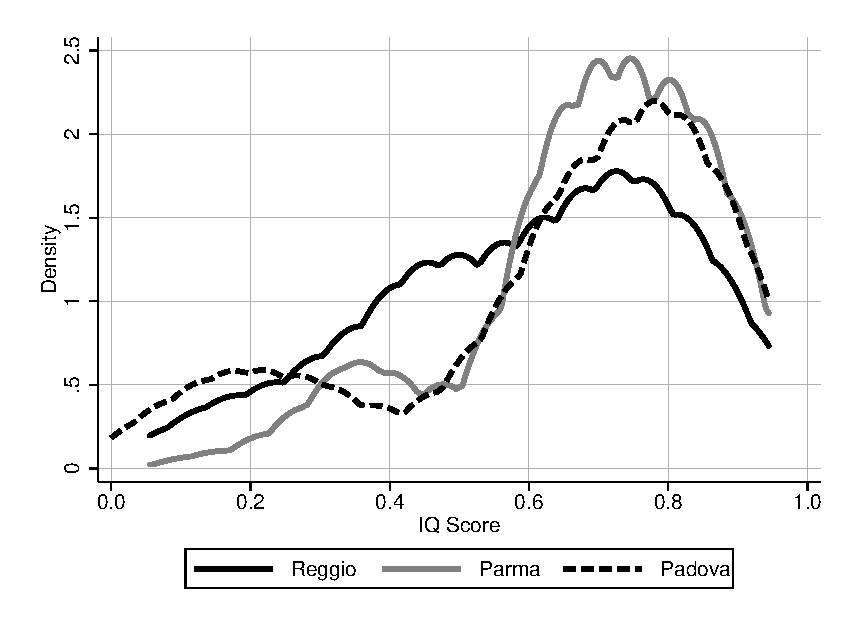
\includegraphics[width=20em]{../../../../Output/IQ_hist_1}
		\caption{Children}
	\end{subfigure}%
	\begin{subfigure}{.5\textwidth}
		\centering
		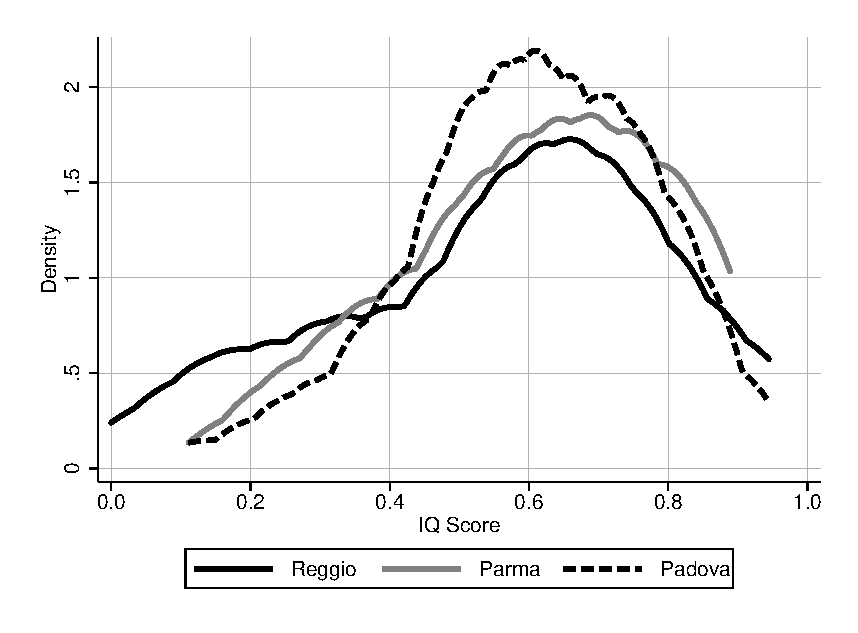
\includegraphics[width=20em]{../../../../Output/IQ_hist_2}
		\caption{Migrants}
	\end{subfigure}
	\begin{subfigure}{.5\textwidth}
		\centering
		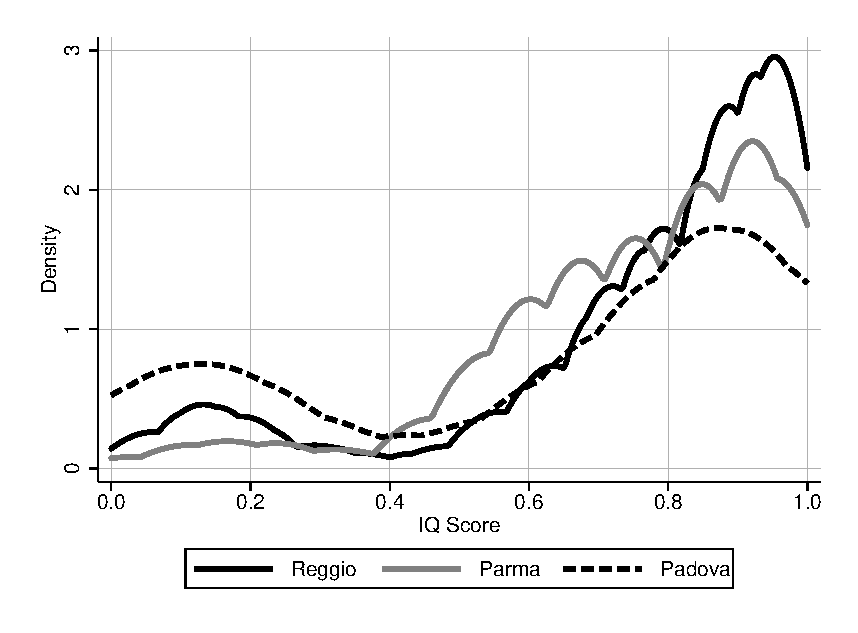
\includegraphics[width=20em]{../../../../Output/IQ_hist_3}
		\caption{Adolescents}
	\end{subfigure}%
	\begin{subfigure}{.5\textwidth}
		\centering
		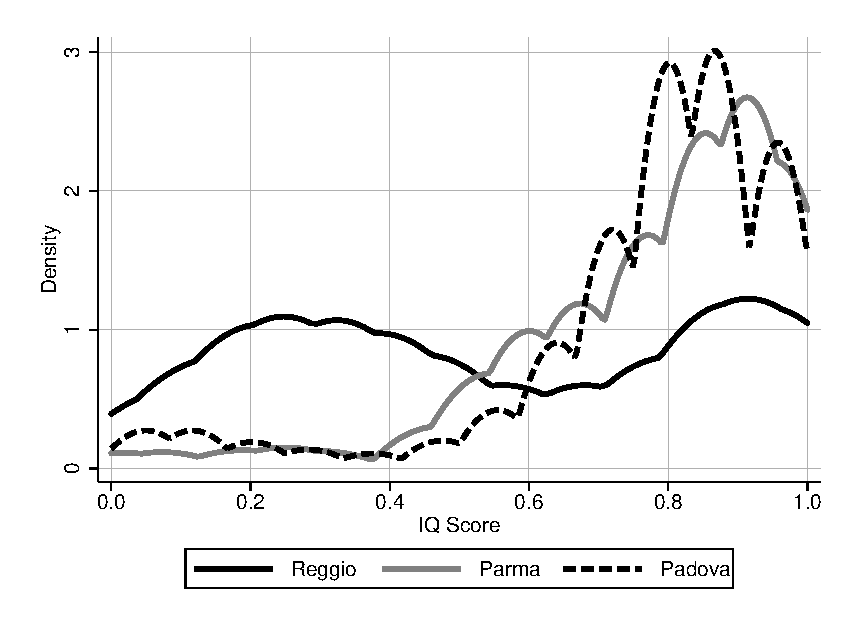
\includegraphics[width=20em]{../../../../Output/IQ_hist_4}
		\caption{Adults 30s}
	\end{subfigure}
	\begin{subfigure}{.5\textwidth}
		\centering
		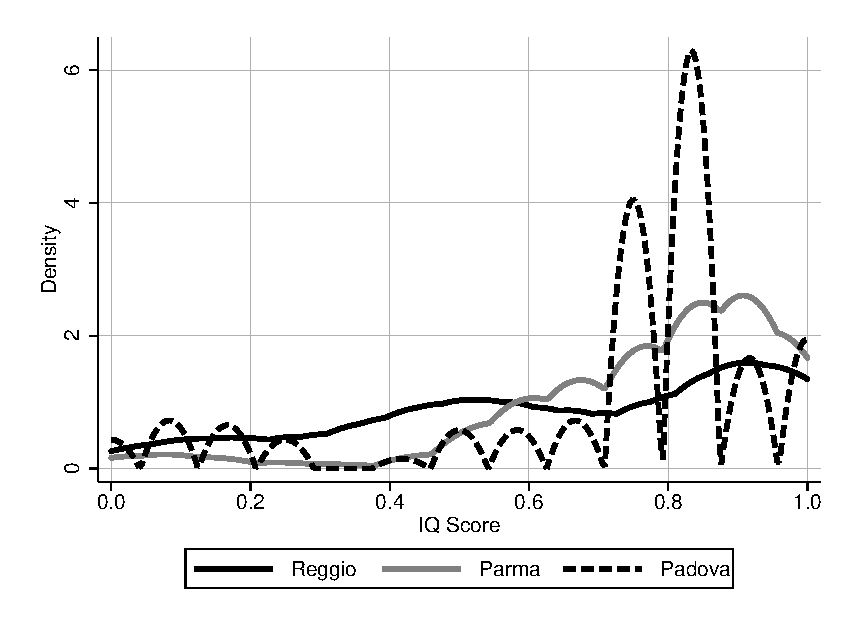
\includegraphics[width=20em]{../../../../Output/IQ_hist_5}
		\caption{Adults 40s}
	\end{subfigure}%
	\begin{subfigure}{.5\textwidth}
		\centering
		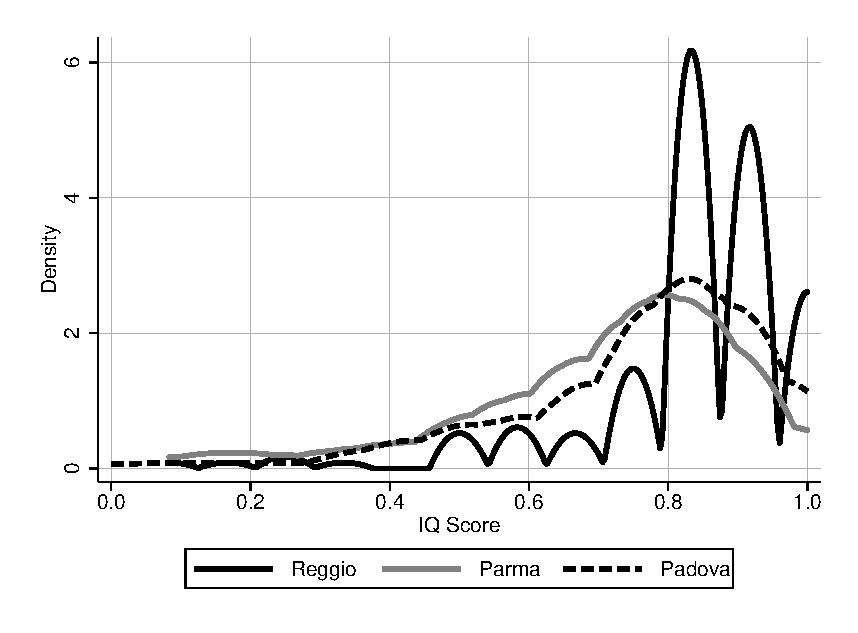
\includegraphics[width=20em]{../../../../Output/IQ_hist_6}
		\caption{Adults 50s}
	\end{subfigure}
\end{center}
\raggedright \footnotesize
Note: These plots show the distributions of IQ scores by city and cohort. The distributions of the different cities are more similar for the younger cohorts than for the adult cohorts. 
\end{figure}


\clearpage

\begin{landscape}
\begin{table}[htbp]
	% created using descriptive.do
\singlespace
\setlength{\tabcolsep}{2pt}
\begin{center}
\scriptsize{
\begin{longtable}{L{12em} c c c p{1.2em} c c c p{1.2em} c c c p{1.2em} c c c p{1.2em} c c c p{1.2em} c c c}
\hline\multicolumn{24}{L{20cm}}{\textbf{Note:} Unconditional means are reported for each variable by cohort and city. Standard Deviations are reported in italics below each mean estimates.}
\endfoot
\caption{Mean and Standard Deviation for Education variables by city and cohort} \label{table:Desc_E} \\
\hline
& \multicolumn{3}{c}{\textbf{Children}} & & \mc{3}{c}{\textbf{Migrants}} & & \multicolumn{3}{c}{\textbf{Adolescents}} & & \multicolumn{3}{c}{\textbf{Adults 30}} & & \multicolumn{3}{c}{\textbf{Adults 40}} & & \multicolumn{3}{c}{\textbf{Adults 50}}\\
& \scriptsize{Reggio} & \scriptsize{Parma}& \scriptsize{Padova} & & \scriptsize{Reggio} & \scriptsize{Parma}& \scriptsize{Padova} & & \scriptsize{Reggio} & \scriptsize{Parma}& \scriptsize{Padova} & & \scriptsize{Reggio} & \scriptsize{Parma}& \scriptsize{Padova} & & \scriptsize{Reggio} & \scriptsize{Parma}& \scriptsize{Padova} & & \scriptsize{Reggio} & \scriptsize{Parma}& \scriptsize{Padova}\\
\hline \\ \endhead \\
IQ Score & 0.60 &      0.69 &      0.64 & &      0.56 &      0.61 &      0.60 & &      0.77 &      0.76 &      0.65 & &      0.57 &      0.78 &      0.78 & &      0.66 &      0.77 &      0.72 & &      0.84 &      0.71 &      0.77 \\*
& $\mathit{     0.22}$ & $\mathit{     0.18}$ & $\mathit{     0.24}$ & & $\mathit{     0.24}$ & $\mathit{     0.19}$ & $\mathit{     0.17}$ & & $\mathit{     0.25}$ & $\mathit{     0.21}$ & $\mathit{     0.34}$ & & $\mathit{     0.33}$ & $\mathit{     0.21}$ & $\mathit{     0.22}$ & & $\mathit{     0.29}$ & $\mathit{     0.22}$ & $\mathit{     0.25}$ & & $\mathit{     0.15}$ & $\mathit{     0.20}$ & $\mathit{     0.19}$ \\[.7em]
IQ Factor & -0.07 &      0.26 &      0.01 & &     -0.31 &     -0.05 &     -0.19 & &      0.15 &      0.16 &     -0.30 & &     -0.19 &      0.47 &      0.43 & &      0.09 &      0.45 &      0.31 & &      0.58 &      0.32 &      0.45 \\*
& $\mathit{     0.93}$ & $\mathit{     0.79}$ & $\mathit{     1.08}$ & & $\mathit{     1.02}$ & $\mathit{     0.80}$ & $\mathit{     0.75}$ & & $\mathit{     0.85}$ & $\mathit{     0.67}$ & $\mathit{     1.19}$ & & $\mathit{     0.93}$ & $\mathit{     0.54}$ & $\mathit{     0.62}$ & & $\mathit{     0.80}$ & $\mathit{     0.58}$ & $\mathit{     0.76}$ & & $\mathit{     0.40}$ & $\mathit{     0.57}$ & $\mathit{     0.48}$ \\[.7em]
Caregiver IQ Score & 0.64 &      0.76 &      0.72 & &      0.47 &      0.61 &      0.50 & &      0.74 &      0.75 &      0.65 & &         . &         . &         . & &         . &         . &         . & &         . &         . &         . \\*
& $\mathit{     0.29}$ & $\mathit{     0.21}$ & $\mathit{     0.29}$ & & $\mathit{     0.27}$ & $\mathit{     0.23}$ & $\mathit{     0.27}$ & & $\mathit{     0.26}$ & $\mathit{     0.22}$ & $\mathit{     0.33}$ & & $\mathit{        .}$ & $\mathit{        .}$ & $\mathit{        .}$ & & $\mathit{        .}$ & $\mathit{        .}$ & $\mathit{        .}$ & & $\mathit{        .}$ & $\mathit{        .}$ & $\mathit{        .}$ \\[.7em]
Caregiver IQ Factor & -0.04 &      0.35 &      0.18 & &     -0.61 &     -0.11 &     -0.58 & &      0.09 &      0.17 &     -0.26 & &         . &         . &         . & &         . &         . &         . & &         . &         . &         . \\*
& $\mathit{     0.96}$ & $\mathit{     0.64}$ & $\mathit{     0.96}$ & & $\mathit{     0.95}$ & $\mathit{     0.78}$ & $\mathit{     0.91}$ & & $\mathit{     0.87}$ & $\mathit{     0.68}$ & $\mathit{     1.16}$ & & $\mathit{        .}$ & $\mathit{        .}$ & $\mathit{        .}$ & & $\mathit{        .}$ & $\mathit{        .}$ & $\mathit{        .}$ & & $\mathit{        .}$ & $\mathit{        .}$ & $\mathit{        .}$ \\[.7em]
High School Grade & . &         . &         . & &         . &         . &         . & &     76.44 &     80.71 &     82.63 & &     82.86 &     74.16 &     77.89 & &     83.36 &     74.98 &     78.66 & &     79.89 &     72.47 &     75.91 \\*
& $\mathit{        .}$ & $\mathit{        .}$ & $\mathit{        .}$ & & $\mathit{        .}$ & $\mathit{        .}$ & $\mathit{        .}$ & & $\mathit{    12.13}$ & $\mathit{    12.05}$ & $\mathit{    10.64}$ & & $\mathit{     9.20}$ & $\mathit{    18.32}$ & $\mathit{    14.42}$ & & $\mathit{     8.22}$ & $\mathit{    14.91}$ & $\mathit{    11.25}$ & & $\mathit{     8.80}$ & $\mathit{    14.79}$ & $\mathit{    11.77}$ \\[.7em]
University Grade & . &         . &         . & &         . &         . &         . & &         . &         . &         . & &    100.67 &     99.68 &     99.81 & &     97.17 &    100.73 &     98.48 & &     97.19 &    100.17 &    104.24 \\*
& $\mathit{        .}$ & $\mathit{        .}$ & $\mathit{        .}$ & & $\mathit{        .}$ & $\mathit{        .}$ & $\mathit{        .}$ & & $\mathit{        .}$ & $\mathit{        .}$ & $\mathit{        .}$ & & $\mathit{     6.38}$ & $\mathit{     7.35}$ & $\mathit{     8.38}$ & & $\mathit{     6.49}$ & $\mathit{     7.52}$ & $\mathit{     7.74}$ & & $\mathit{     6.77}$ & $\mathit{     7.12}$ & $\mathit{     6.66}$ \\[.7em]
Graduate from High School & . &         . &         . & &         . &         . &         . & &         . &         . &         . & &      0.88 &      0.89 &      0.88 & &      0.80 &      0.84 &      0.82 & &      0.74 &      0.59 &      0.57 \\*
& $\mathit{        .}$ & $\mathit{        .}$ & $\mathit{        .}$ & & $\mathit{        .}$ & $\mathit{        .}$ & $\mathit{        .}$ & & $\mathit{        .}$ & $\mathit{        .}$ & $\mathit{        .}$ & & $\mathit{     0.33}$ & $\mathit{     0.31}$ & $\mathit{     0.32}$ & & $\mathit{     0.40}$ & $\mathit{     0.37}$ & $\mathit{     0.38}$ & & $\mathit{     0.44}$ & $\mathit{     0.49}$ & $\mathit{     0.50}$ \\[.7em]
Max Edu: University & 0.00 &      0.00 &      0.00 & &      0.00 &      0.00 &      0.00 & &      0.00 &      0.00 &      0.00 & &      0.19 &      0.38 &      0.45 & &      0.15 &      0.28 &      0.33 & &      0.11 &      0.12 &      0.23 \\*
& $\mathit{     0.00}$ & $\mathit{     0.00}$ & $\mathit{     0.00}$ & & $\mathit{     0.00}$ & $\mathit{     0.00}$ & $\mathit{     0.00}$ & & $\mathit{     0.00}$ & $\mathit{     0.00}$ & $\mathit{     0.00}$ & & $\mathit{     0.39}$ & $\mathit{     0.49}$ & $\mathit{     0.50}$ & & $\mathit{     0.36}$ & $\mathit{     0.45}$ & $\mathit{     0.47}$ & & $\mathit{     0.31}$ & $\mathit{     0.32}$ & $\mathit{     0.42}$ \\[.7em]
Max Edu: Graduate School & 0.00 &      0.00 &      0.00 & &      0.00 &      0.00 &      0.00 & &      0.00 &      0.00 &      0.00 & &      0.00 &      0.03 &      0.09 & &      0.00 &      0.04 &      0.02 & &      0.00 &      0.00 &      0.05 \\*
& $\mathit{     0.00}$ & $\mathit{     0.00}$ & $\mathit{     0.00}$ & & $\mathit{     0.00}$ & $\mathit{     0.00}$ & $\mathit{     0.00}$ & & $\mathit{     0.00}$ & $\mathit{     0.00}$ & $\mathit{     0.00}$ & & $\mathit{     0.06}$ & $\mathit{     0.16}$ & $\mathit{     0.29}$ & & $\mathit{     0.00}$ & $\mathit{     0.19}$ & $\mathit{     0.15}$ & & $\mathit{     0.00}$ & $\mathit{     0.00}$ & $\mathit{     0.21}$ \\[.7em]
\hline
\end{longtable}
}
\end{center}

\end{table}
\end{landscape}

\begin{landscape}
\begin{table}[htbp]
	% created using descriptive.do
\singlespace
\setlength{\tabcolsep}{2pt}
\begin{center}
\scriptsize{
\begin{longtable}{L{12em} c c c p{1.2em} c c c p{1.2em} c c c p{1.2em} c c c p{1.2em} c c c p{1.2em} c c c}
\multicolumn{24}{L{23cm}}{\textbf{Note:} This table reports the number of observations that are missing for each education variable by city and cohort. \textbf{--} indicates that the variable has 0 observations for the particular cohort-city group.}
\endfoot\caption{Missing observations for education variables by city and cohort} \label{table:Miss_edu} \\
\hline
& \multicolumn{3}{c}{\textbf{Children}} & & \mc{3}{c}{\textbf{Migrants}} & & \multicolumn{3}{c}{\textbf{Adolescents}} & & \multicolumn{3}{c}{\textbf{Adults 30}} & & \multicolumn{3}{c}{\textbf{Adults 40}} & & \multicolumn{3}{c}{\textbf{Adults 50}}\\
& \scriptsize{Reggio} & \scriptsize{Parma}& \scriptsize{Padova} & & \scriptsize{Reggio} & \scriptsize{Parma}& \scriptsize{Padova} & & \scriptsize{Reggio} & \scriptsize{Parma}& \scriptsize{Padova} & & \scriptsize{Reggio} & \scriptsize{Parma}& \scriptsize{Padova} & & \scriptsize{Reggio} & \scriptsize{Parma}& \scriptsize{Padova} & & \scriptsize{Reggio} & \scriptsize{Parma}& \scriptsize{Padova}\\
\hline \endhead \\
IQ Score & 0.00 &      0.00 &      0.00 & &      0.00 &      0.00 &      0.00 & &      0.00 &      0.00 &      0.00 & &      0.00 &      0.00 &      0.00 & &      0.00 &      0.00 &      0.00 & &      0.00 &      0.00 &      0.00 \\[.3em]
IQ Factor & 0.00 &      0.00 &      0.00 & &      0.00 &      0.00 &      0.00 & &      0.00 &      0.00 &      0.00 & &      0.00 &      0.00 &      0.00 & &      0.00 &      0.00 &      0.00 & &      0.00 &      0.00 &      0.00 \\[.3em]
Caregiver IQ Score & 0.00 &      0.00 &      0.00 & &      0.00 &      0.00 &      0.00 & &      0.00 &      0.00 &      0.00 & & - & - & - & & - & - & - & & - & - & - \\[.3em]
Caregiver IQ Factor & 0.00 &      0.00 &      0.00 & &      0.00 &      0.00 &      0.00 & &      0.00 &      0.00 &      0.00 & & - & - & - & & - & - & - & & - & - & - \\[.3em]
High School Grade & - & - & - & & - & - & - & &      0.93 &      0.72 &      0.71 & &      0.23 &      0.12 &      0.19 & &      0.26 &      0.16 &      0.21 & &      0.26 &      0.44 &      0.49 \\[.3em]
University Grade & - & - & - & & - & - & - & & - & - & - & &      0.81 &      0.62 &      0.55 & &      0.85 &      0.72 &      0.67 & &      0.89 &      0.88 &      0.77 \\[.3em]
Graduate from High School & - & - & - & & - & - & - & & - & - & - & &      0.00 &      0.00 &      0.00 & &      0.00 &      0.00 &      0.00 & &      0.00 &      0.00 &      0.00 \\[.3em]
Max Edu: University & 0.00 &      0.00 &      0.00 & &      0.00 &      0.00 &      0.00 & &      0.00 &      0.01 &      0.00 & &      0.00 &      0.00 &      0.00 & &      0.00 &      0.00 &      0.00 & &      0.00 &      0.00 &      0.00 \\[.3em]
Max Edu: Graduate School & 0.00 &      0.00 &      0.00 & &      0.00 &      0.00 &      0.00 & &      0.00 &      0.01 &      0.00 & &      0.00 &      0.00 &      0.00 & &      0.00 &      0.00 &      0.00 & &      0.00 &      0.00 &      0.00 \\[.3em]
\hline
\end{longtable}
}
\end{center}

\end{table}
\end{landscape}
\section{Education Variables}
\label{sec:edu}
\subsection{Maximum Education}

Maximum education variable has 9 categories, which are shown in Table \ref{tab:par-maxedu}. Since Italian education system has experienced changes in 1999 due to Bologna process\footnote{Bologna process is a series of ministerial meetings and agreements between European countries designed to ensure comparability in the standards and quality of higher education qualifications.}, those need to be accounted for when converting the education categories into years of education. Column 3 of Table \ref{tab:par-maxedu} shows the converted years of education according to information below. 

Italian elementary school (Scuola elementare) lasts 5 years. We assume that all parents for younger cohorts attended elementary school unless noted otherwise. ``Scuola media inferiore" last for 3 years (roughly from age 11 to 13). There are two types of high school listed in our category. ``Biennio scuola media superiore" offers two years of education and the ``Scoula media superiore" offers 4 or 5 years of education. 

After the Bologna agreement, most of universities in Italy became a 3+2 system, each period granting a certification. First 3 years (laurea triennale) can be considered as a bachelors, and the second 2 years (laurea biennale) can be translated as a masters program. However, in reality, 3+2 is same as previous university degree (diploma universitario). Because of the timing when this change took place, these years of education does not apply to age-40 and age-50 cohorts in the Reggio data. 

There are some difference in how degrees are called in Italy and in the United States. ``Laurea specialistica o magistrale" in our category, although it is translated as ``master", is more similar to bachelor's in the United States. On the other hand, ``master post-laurea", which includes MBA, can be considered as the actual master's degree. 


\begin{table}[H]
\caption{Categories for Parental Maximum Education} \label{tab:par-maxedu}
\begin{center}
\begin{tabular}{L{4.3cm} L{4.3cm} L{4.3cm}}
\toprule
\textbf{Italian Label} & \textbf{English Label} & \textbf{Years of Education} \\ \midrule
	(1) Scuola media inferiore/licenza elementa &	Junior High School/Primary School		& 8 years \\
	(2) Biennio scuola media superiore & 				Two years high school								& 10 years \\
	(3) Scuola media superiore (4 o 5 anni) & 		High School (4 or 5 years)								& 12 years \\
	(4) Diploma universitario &	University Diploma & 16 years \\
	(5) Laurea triennale &	Three-year Degree &	15 years \\
	(6) Laurea quadriennale/quinquennale &   	Five-year Degree & 17 years \\
	(7) Laurea specialistica o magistrale & 			Master & 17 years \\
	(8) Master post-laurea quadr./quinq./sp  & Master postgraduate framework			& 19 years \\
	(9) Dottorato di ricerca 	& Ph.D.	& 23 years \\ \bottomrule
\end{tabular}
\end{center}
\end{table}

\subsection{High School Grades}
High school grade (votoMaturita) that was asked in the questionnaires has two different scales, one has the maximum scoring of 60 and the other has 100. The former scale is the old scoring scheme that was changed to latter by the law n.1/2007. Before 2007, the maximum grade was 60 and the minimum passing grade was 36 (below 36 was fail). After 2007, the maximum grade became 100 and the minimum passing grade became 60 (below 60 is fail)\footnote{http://www.classbase.com/Countries/italy/Grading-System}.

Since adolescent cohort went to high school after the change in scoring system, the questionnaire for adolescents asks respondents to provide their high school grades in 100 scale. On the other hand, since people the adult cohorts might have used 60 scale when they attended high school, the questionnaire for adults ask respondents two different choices (old way and new way) to report their high school grade. Grades reported in the 60 scale are converted to the 100 scale. 

Table \ref{tab:hsgrade} shows the high school types listed in the questionnaire and mean high school grade for each school type in each city. Across all three cities, majority of people attended either classic high school, science high school, or technical institute, which is specialized in surveyor, accountancy, industrial, etc. Reggio's mean high school grade is generally higher than Parma and Padova across all school types. In Reggio, institutes for socio-psycho-pedagogy exhibit the highest mean grade and professional schools exhibit the lowest mean grade. In Parma, art, music, or choir school has the highest mean grade, and institute for socio-psycho-pedagogy shows the lowest mean grade. In Padova, language high schools show the highest mean grade, and art, music, or choir school show the lowest mean grade.

\begin{table}[H]
\caption{Mean High School Grade for Each High School Type} \label{tab:hsgrade}
\begin{center}
\footnotesize
\begin{tabular}{lllll}
\toprule
  & \textbf{Reggio} & \textbf{Parma} & \textbf{Padova}  & \textbf{Total} \\ \midrule
\textbf{Classic high school}  \\
\quad Mean  & 82.27 &  75.51 &  78.69 & 79.25 \\ 
         \quad SE & 10.22 & 15.05 & 14.05 & 13.16 \\
         \quad N  &  121   &      87    &     69 &       277 \\

\textbf{Science high school} \\ 
 \quad Mean & 84.17 &  78.34 &      79.45 & 80.43 \\
  \quad SE & 8.65 & 16.34 & 13.79 & 13.64 \\
   \quad N  &       109   &     119    &    160   &      388 \\ 

\textbf{Language high school}  \\ 
 \quad Mean & 83.52  &  80.97   &   83.35  & 82.36 \\
 \quad SE & 8.78 & 11.71  & 10.78 & 10.54 \\
  \quad N &    34     &    43    &     20   &        97 \\ 

\textbf{Art, music, or choir school}  \\ 
 \quad Mean & 84.57 &  87.88 &  73.55 &      81.8 \\
  \quad SE & 6.50 &  10.44 &   8.57 & 10.63 \\
  \quad N &   7     &     9    &      9 &        25 \\ 

\textbf{Institute for socio-psycho-pedagogy}  \\ 
 \quad Mean & 86.88 &      70.1 & 79.26 & 78.58 \\
  \quad SE & 14.13 &   26.01  & 16.26 & 19.65 \\
  \quad N &    9  &       10   &      15 &        34 \\ 

\textbf{Conservatory}  \\ 
 \quad Mean &        83      &   83   &      75 &        81 \\
 \quad SE &         0       &   0    &      0 &         4 \\
 \quad N &         2        &  1     &     1 &         4 \\ 

\textbf{Technical Institute}  \\ 
 \quad Mean & 82.05 &  70.95 &  76.76 & 76.75 \\
 \quad SE & 7.94 & 16.27 &  11.24 &  12.95  \\
  \quad N &       204 &       187 &       206 &       597 \\ 

\textbf{Professional (chemical, electronic, etc.)}  \\ 
 \quad Mean & 78.85 & 75.84 &    79.87 & 78.20 \\
  \quad SE & 7.62 & 9.07 &  13.36 & 9.28 \\
  \quad N &        76 &        38 &        24 &       138 \\ 

\textbf{Art institute}  \\ 
 \quad Mean & 79.07 &      78.2 & 74.85 &      77.8 \\
 \quad SE & 9.88 & 19.34 & 6.54 &  12.97 \\
 \quad N &        13 &        10 &         7 &        30 \\ 

\textbf{Other}  \\ 
  \quad Mean &         . &     71.75 &         . &     71.75 \\
  \quad SE &         . & 5.67 &         . & 5.67 \\
  \quad N &         0 &         4 &         0 &         4 \\ \bottomrule

\end{tabular}
\end{center}
\end{table}
\normalsize

\section{Cognitive Variables}
\label{sec:cog}

IQ is measured for all individuals in the sample as well as for the caregivers of the children, migrants, and adolescents using Raven's Progressive Matrices (Raven's).\footnote{\citet{Raven_Raven_etal_1988_BOOKManualRavensprogressive}.} Raven's is a non-verbal test that is correlated with other measures of fluid intelligence. The 12-Item and 18-Item versions are shortened from the original version, which helps reduce the duration of the test. Both shortened versions are highly correlated with the full version of the test, which in turn is highly correlated with other measures of IQ.

Each item on the test consists of a matrix of diagrams that follow some logical pattern with one missing diagram that the test-taker needs to select from multiple choices. A correct answer is assigned a value of 1, and an incorrect answer is assigned a value of 0. The IQ score is the proportion of questions answered correctly. If questions are missed, then they do not count in the total number of questions. The factor scores are computed using a specification of a structural equation using maximum likelihood that accounts for missing values. That is, it requires the assumption that bot the observed and latent variables are jointly distributed normally, and that any missing values are missing at random. The latter assumption is the more tenuous assumption given that a missing item could mean the individual could not answer the question at all due to lower cognitive ability (as opposed to rushing through the test or inability to focus).
% The variables that measure these binary item-level responses for subjects are IQ*. For caregivers, the analogous variables are cgIQ*.

 Table \ref{tab:test-type} explains which individuals in which cohort received the 12- or 18-Item version of Raven's Progress Matrices (Raven's).

\begin{table}[H]
\begin{center}
	\caption{IQ Test by Cohort}\label{tab:test-type}
	\begin{tabular}{lcc}
		\toprule
		Cohort & 12-Item & 18-Item \\
		\midrule
		\textbf{Children} & &\\
		\quad Subjects & & $\checkmark$  \\
		\quad Caregivers &  $\checkmark$ & \\
		\textbf{Migrants} & & \\
		\quad Subjects & & $\checkmark$ \\
		\quad Caregivers & $\checkmark$ &  \\
		\textbf{Adolescents} & & \\
		\quad Subjects & $\checkmark$ & \\
		\quad Caregivers &  $\checkmark$ &  \\
		\textbf{Adults} & & \\
		\quad Subjects & & $\checkmark$ \\
		\bottomrule
	\end{tabular}
\end{center}
\raggedright \footnotesize Note: This table shows the type of test given for each cohort. The caregivers were always given the 12-Item Raven's. The 18-Item Raven's was only meant for younger subjects (the individuals in the children and migrants cohorts were about 6 years old at the time of the test).
\end{table}

Figure \ref{fig:iq-hist} shows the distribution of the IQ score by city and cohort. 

\begin{figure}[H]
	\begin{center}
	\caption{Densities of IQ Scores}\label{fig:iq-hist}
	\begin{subfigure}{.5\textwidth}
		\centering
		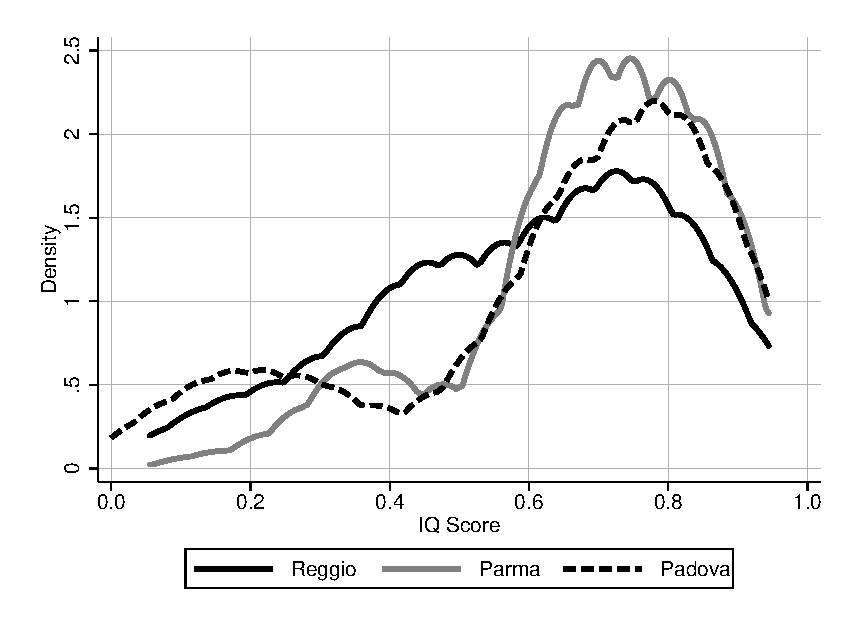
\includegraphics[width=20em]{../../../../Output/IQ_hist_1}
		\caption{Children}
	\end{subfigure}%
	\begin{subfigure}{.5\textwidth}
		\centering
		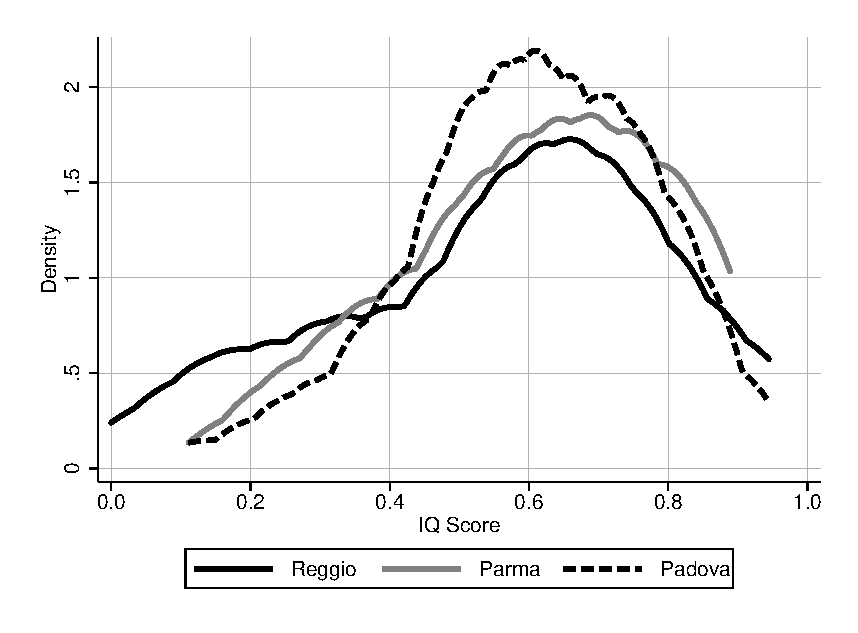
\includegraphics[width=20em]{../../../../Output/IQ_hist_2}
		\caption{Migrants}
	\end{subfigure}
	\begin{subfigure}{.5\textwidth}
		\centering
		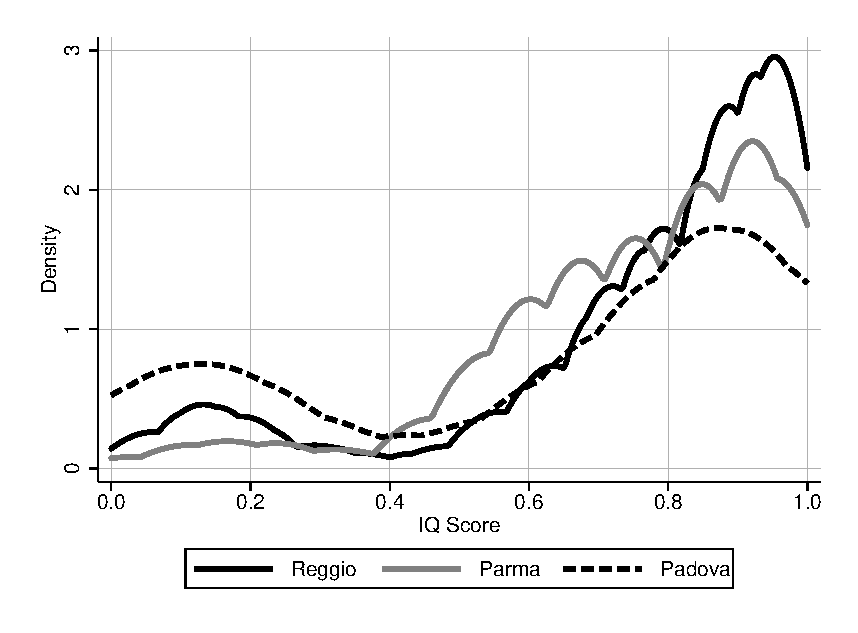
\includegraphics[width=20em]{../../../../Output/IQ_hist_3}
		\caption{Adolescents}
	\end{subfigure}%
	\begin{subfigure}{.5\textwidth}
		\centering
		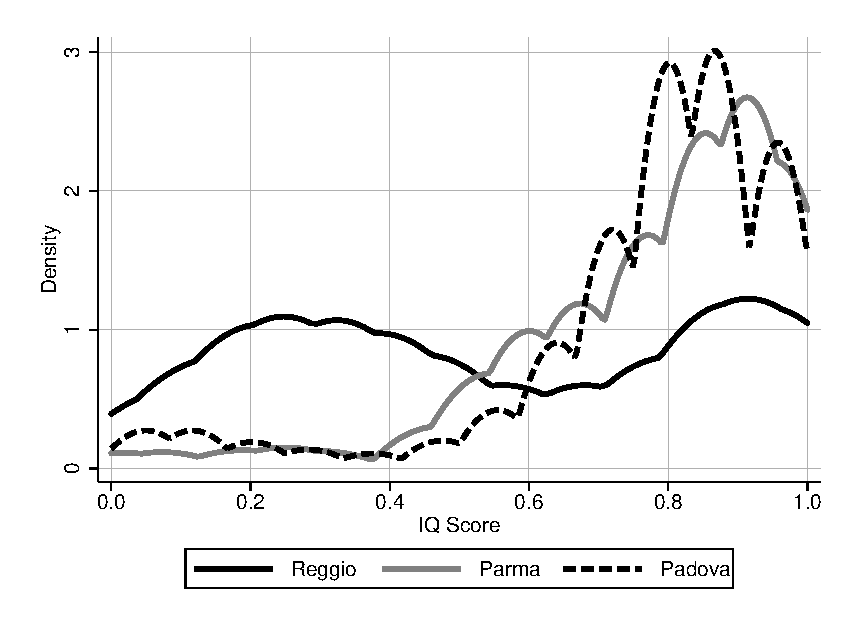
\includegraphics[width=20em]{../../../../Output/IQ_hist_4}
		\caption{Adults 30s}
	\end{subfigure}
	\begin{subfigure}{.5\textwidth}
		\centering
		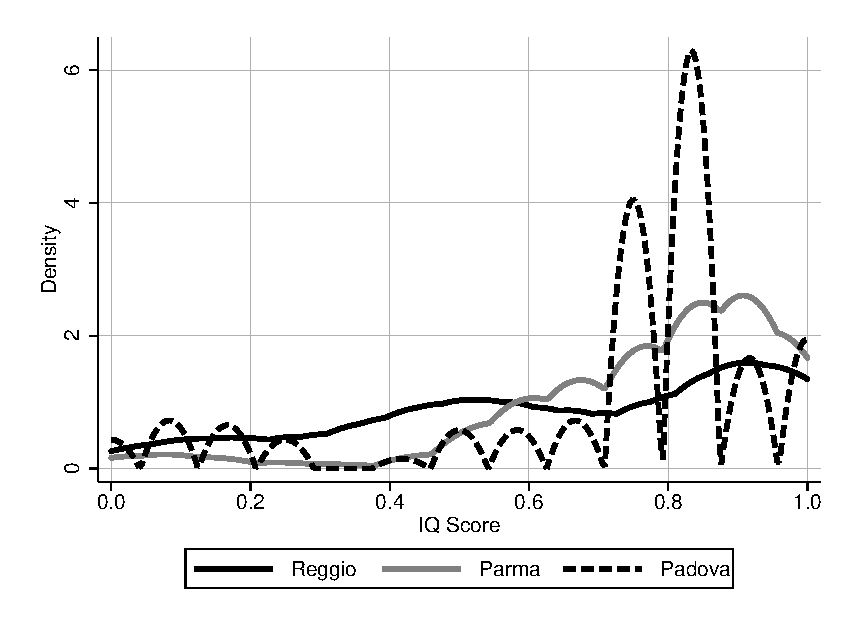
\includegraphics[width=20em]{../../../../Output/IQ_hist_5}
		\caption{Adults 40s}
	\end{subfigure}%
	\begin{subfigure}{.5\textwidth}
		\centering
		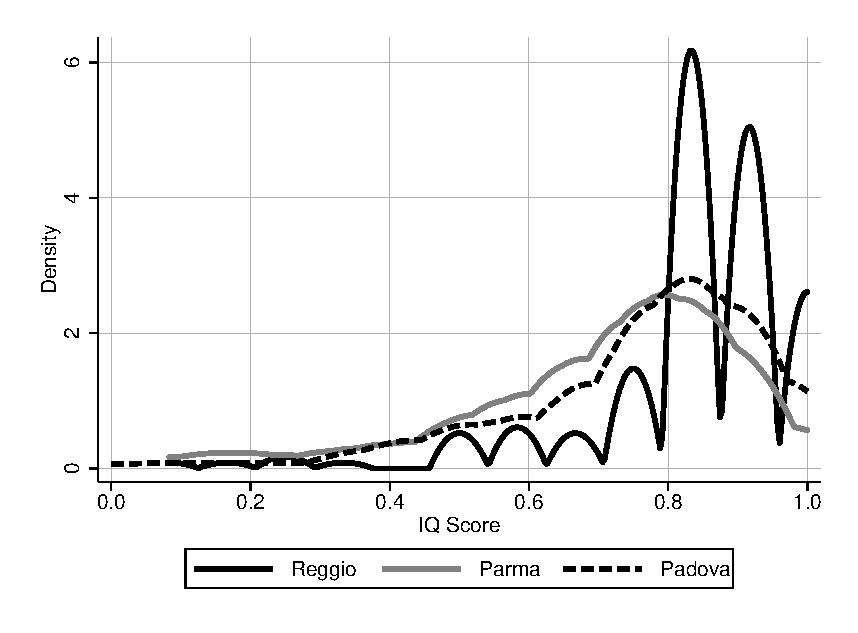
\includegraphics[width=20em]{../../../../Output/IQ_hist_6}
		\caption{Adults 50s}
	\end{subfigure}
\end{center}
\raggedright \footnotesize
Note: These plots show the distributions of IQ scores by city and cohort. The distributions of the different cities are more similar for the younger cohorts than for the adult cohorts. 
\end{figure}


\section{Income and Employment Variables}
\label{sec:income}
\subsection{Family Income}

Table \ref{tab:faminc} lists categories of income in our questionnaire. This category is used for (i) baseline family income and (ii) current family income. Although (i) and (ii) are measuring income at different point of time with different inflation rates, since the questions that were asked does not account for the inflation rate, we do not account for inflation rate when converting categories into values. We apply median of reported category when creating income variables shown in values. 

\begin{table}[H]
\caption{Categories for Family Income} \label{tab:faminc}
\begin{center}
\begin{tabular}{ll}
\toprule
\textbf{Category} & \textbf{Value} \\ \midrule
	1 - 5,000 Euro					 & 2,500 Euro \\
	5,001 - 10,000 Euro				 & 7,500 Euro \\
	10,001 - 25,000 Euro			 & 17,500 Euro \\
	25,001 - 50,000 Euro			 & 37,500 Euro \\
	50,001 - 100,000 Euro			 & 75,000 Euro \\
	100,001 - 250,000 Euro			 & 175,000 Euro \\
	More than 250,000 Euro			 & 375,000 Euro \\ \bottomrule
\end{tabular}
\end{center}
\end{table}
	
\subsection{Caregiver's Occupation and Hours of Work}
Caregiver's occupation variable has 12 categories in the questionnaire: (i) never worked, (ii) farmer, (iii) worker, (iv) employee, (v) teacher, (vi) executive, (vii) manager, (viii) professional (doctor, lawyer, etc.), (ix) entrepreneur, (x) self-employed, (xi) atypical worker, (xii) other.  

There are two measures of caregiver's hours of work in the questionnaire: (i) normal hours of work per week and (ii) average overtime hours per week. Caregiver's total hours of work per week is computed by combining normal hours and overtime hours. Moreover, if a caregiver reported to have ``never worked" when reporting occupation, we record the total hours of work for such caregiver as 0 hours. The mean total hours of work of caregiver is  34.57 hours with the standard error 12.99. The minimum weekly hours of worked is 0 hour and the maximum is 90 hours in the data.

\subsection{House Ownership}
The question that asks "Is this house owned by this household?" is both for parents of children and adolescents and for adults. This means that for younger cohorts, this variable shows the ownership of their caregivers. For adult cohorts, this variable shows whether respondent owns house. 

\section{Health Variables}
\label{sec:health}


\section{Instruments}
\label{sec:instruments}

% Commenting this until it becomes complete.
%\subsection{Distance as Instrumental Variable}
%Fourteen instrumental variables have been contructed that measure the distance from each individual's house to the two nearest municipal, state, religious, and private schools in both \textit{asilo} and \textit{materna} categories. The data contains (i) a variable that records respondent's self-reported home address, and (ii) information including name, address, and years of operation of 372 \textit{asilo} and \textit{materna} school. ArcGIS is used to generate exact coordinates for each house and school address from this data. These coordinates are used to calculate geodetic distances from each individual's house to every school in the data. The two smallest distances for each school type is stored and used as instrumental variables. 



\singlespace
\bibliographystyle{chicago}
\bibliography{heckman}
\end{document}